\subsubsection{Well management service}


The \textit{WellManagementService} is a high-level interface designed for creating multiple wells simultaneously. Its structure allows seamless integration with the API.
The service loads wells from a JSON configuration file, constructs them, and returns a \textit{WellManagementServiceResult} model, which can easily be serialized into a JSON file or a Python dictionary object. The class supports well shapes of types I, J, and S. Additionally, perforations can be defined for each well.\\\\
\textbf{Workflow}\\
The workflow of the \textit{WellManagementService} begins with providing a configuration file. After validating the configuration, the service initializes a \textit{WellBuilder} object for each well, passing all necessary parameters such as the well's name, sections, perforations, azimuth, and wellhead location.
The \textit{WellBuilder} starts by creating an empty \textit{Trajectory} object. It then iteratively extends the trajectory by adding discretized sections one by one.\\\\
\textit{Note: The initial well trajectory is two-dimensional. The Y-coordinate for every \textit{TrajectoryPoint} is set to zero, and the wellhead of the trajectory is positioned at the origin of the coordinate system. These assumptions simplify well building process.}\\\\
Once all sections have been discretized, the trajectory is rotated to match the configured azimuth. Afterward, the rotated trajectory is translated to the desired location.\\
Each \textit{WellBuilder} instance returns a \textit{Well} object, which includes the trajectory and all perforations assigned to the well. The \textit{WellManagementService} collects all \textit{Well} objects and transforms them into a \textit{WellManagementServiceResult}.\\
To better illustrate this process, the following figure is provided:\\

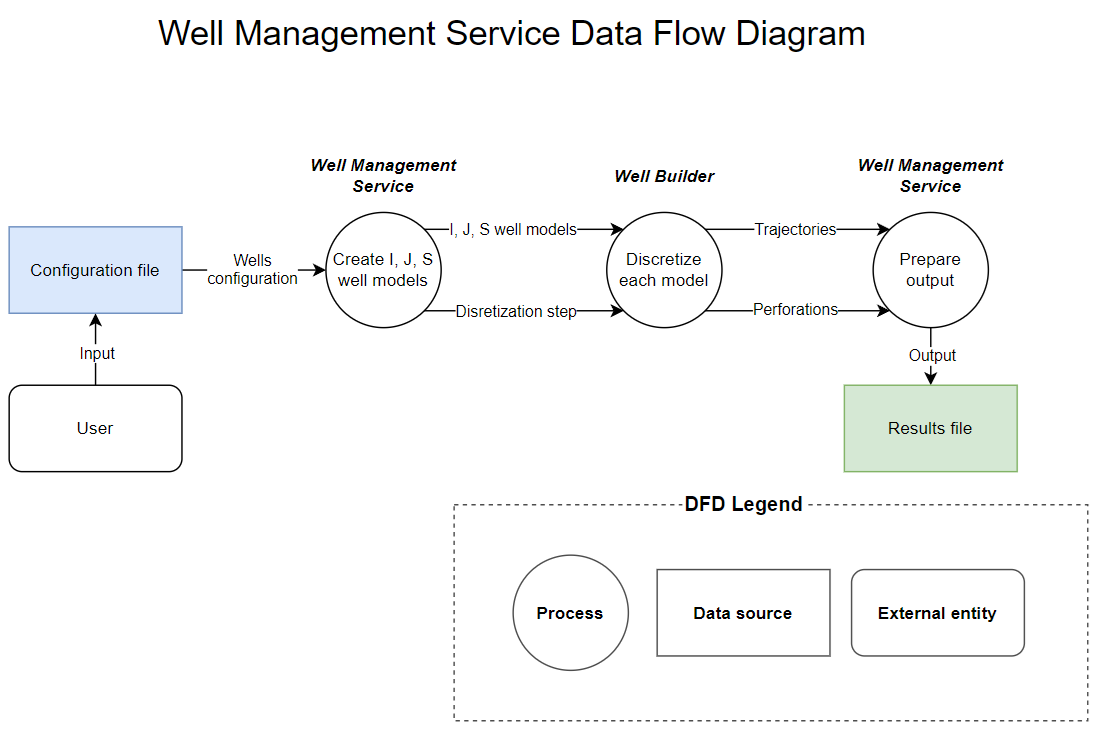
\includegraphics[width=1.0\textwidth]{images/well_management_service/WMS_Data-Flow-Diagram.png}

\subsubsection{Methods}

\begin{description}

\item[ \colorbox{gray!20}{from\_dict}] \hfill
\begin{description}
\item[Arguments:] \hfill
\begin{itemize}
    \item \texttt{config\_dict} (\texttt{dict}) - configuration object format.\\
    %todo: maybe provide config_dict schema
    Sample configuration\\
    \begin{lstlisting}
{
"models": [
{
	"well_type": "IWell",
	"name": "I Sample",
	"md": 100,
	"wellhead": {
		"x": 0.0,
		"y": 0.0,
		"z": 0.0},
	"md_step": 1.0,
	"perforations": [
		{
			"start_md": 10.0,
			"end_md": 60.0},
		{
			"start_md": 70.0,
			"end_md": 80.0},
	],
},
{
	"well_type": "JWell",
	...
},
{
	"well_type": "SWell",
	...
},
{
	"well_type": "HWell",
	...
}
]
}
\end{lstlisting}
    \end{itemize}
        \item[Returns:] \hfill
        \begin{itemize}
            \item \texttt{WellManagementServiceResult} - a collection of wells.
        \end{itemize}
    \end{description}
    \item[\colorbox{gray!20}{dump\_results\_schema}] \hfill
    \begin{description}
        \item[Arguments:] \hfill
        \begin{itemize}
            \item \texttt{path} (\texttt{PathLike}) - path to the file where schema should be dumped.
        \end{itemize}
    \end{description}
\end{description}
